% Chapter 2

\chapter{Radares Passivos} % Main chapter title

\label{chap:Chapter2} % For referencing the chapter elsewhere, use \ref{chap:Chapter2} 

%----------------------------------------------------------------------------------------

\section{Contextualização} \label{contextualização}
Os radares convencionais são constituídos por um transmissor e um recetor, normalmente no mesmo local. Neste tipo de radares, um impulso é transmitido em forma de energia eletromagnética, e através do conhecimento do tempo levado pelo pulso a ser transmitido e recebido depois de refletido no alvo e da velocidade de propagação da luz, consegue-se determinar um valor de distância.\par 
Num radar passivo, não existe transmissão de energia eletromagnética durante o seu funcionamento. Ao invés, utiliza iluminadores de oportunidade e compara o seu sinal direto com pequenas alterações que ocorrem no campo eletromagnético por alvos em movimento de forma a detetar um alvo \parencite{Griffiths2017}.\par 
Este sistema radar pode utilizar uma grande variedade de iluminadores, desde sistemas de navegação por satélite (\textit{\gls{GNSS}}) como o \gls{GPS} ou o GLONASS, \textit{routers} de WiFi ou qualquer sistema de transmissão de frequências rádio como \textit{\gls{DVB}} ou estações de rádio. Assim, por forma a dimensionar o sistema para o efeito desejado, torna-se necessário uma boa compreensão das mais diversas caraterísticas dos iluminadores, como é referido mais à frente neste capítulo.\par 
Para a finalidade de deteção de alvos a grandes distâncias, os sinais mais eficazes e consequentemente mais utilizados são os que apresentam elevada potência, como transmissores de \gls{VHF} e de televisão digital em \gls{UHF}, não obstante poder-se também utilizar em certos casos outros iluminadores.\par
O cenário típico de um esquema de deteção usando um radar passivo é, como ilustrado na Figura \ref{fig:esquema_pcl}, constituído por duas antenas recetoras, uma antena que recebe o sinal direto do iluminador ($S_{ref}$) e outra antena que recebe o sinal que é refletido no alvo ($S_{r}$). O sinal refletido no alvo fornece duas informações importantes para a sua deteção: o \textit{bistatic range}, ou seja, a distância ao alvo, conseguida através da diferença de tempo entre o sinal direto e o sinal refletido; e o \textit{Doppler}, que é o desvio de frequência que um alvo em movimento cria no sinal que é refletido devido à sua velocidade. Estes conceitos são discutidos mais à frente neste capitulo. \par

\begin{figure}[h]
\centering
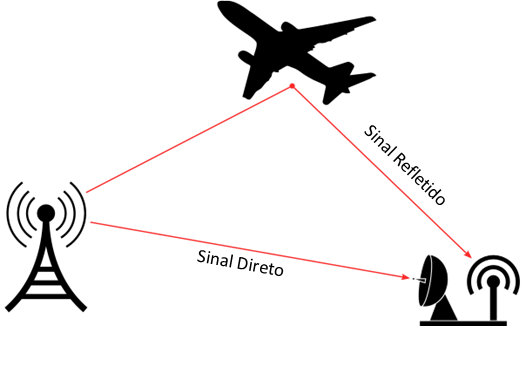
\includegraphics[scale=0.7]{chapters/ch2/assets/esquema_pcl}
\caption[Esquema Geometria Radar Passivo]{Esquema da geometria de um radar passivo}
\label{fig:esquema_pcl}
\end{figure}

O radar passivo consiste em efetuar a relação cruzada (\textit{cross-correlation}) entre o sinal direto e o sinal refletido em função das variáveis \textit{delay-time} (ou \textit{bistatic range}) e o desvio de \textit{Doppler}. A \textit{cross-correlation}, de forma simples, é uma medida de similaridade entre dois sinais aplicando um atraso num deles, que neste caso, para além do atraso em tempo(\textit{delay-time}), também é feita para os diferentes desvios de \textit{Doppler}, ou seja, em duas dimensões. No entanto, na prática existem processos analíticos mais eficientes, visto que fazer a relação cruzada a duas dimensões em tempo real torna o processo muito pesado computacionalmente.



\subsection{Geometrias Radar}
Podemos classificar os radares quanto à localização dos transmissores e recetores. O ângulo $\beta$ que estes formam, sendo o seu centro o alvo, determina o tipo de geometria \parencite{Baker2019}. Se $\beta <20^{\circ}$, considera-se que o transmissor e o recetor se encontram perto ou no mesmo local, podendo então ser aproximada a uma geometria monostática (Figura \ref{fig:monostatic}). Quando o transmissor e recetor estão mais afastados e formam um ângulo com centro no recetor dentro dos seguintes limites, $20^{\circ}<\beta <145^{\circ}$, considera-se a geometria bistática (Figura \ref{fig:bistatic}). Para situações particulares, considera-se que o alvo se encontra a uma cota baixa em relação à linha imaginária que une o transmissor e o recetor ($145^{\circ}<\beta <180^{\circ}$), podendo então ser aproximada a uma geometria \textit{Forward Scatter} (Figura \ref{fig:fsc}).\par   

\begin{figure}[h]
\centering
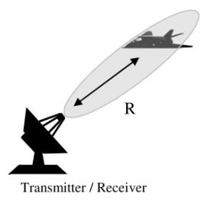
\includegraphics[scale=0.8]{chapters/ch2/assets/monostatic}
\caption[Geometria Monostática]{Geometria Monostática(extraído de \cite{rcsan})}
\label{fig:monostatic}
\end{figure}

\begin{figure}[h]
\centering
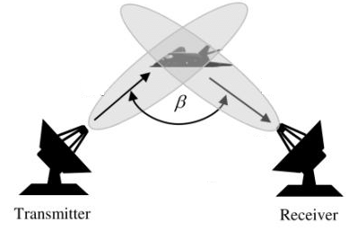
\includegraphics[scale=0.8]{chapters/ch2/assets/bistatic}
\caption[Geometria Bistática]{Geometria Bistática(extraído de \cite{rcsan})}
\label{fig:bistatic}
\end{figure}

\begin{figure}[h]
\centering
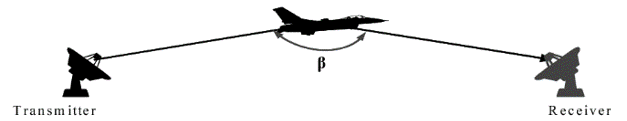
\includegraphics[scale=0.7]{chapters/ch2/assets/fsc}
\caption[Geometria \textit{Forward Scatter}]{Geometria \textit{Forward Scatter}(extraído de \cite{rcsan})}
\label{fig:fsc}
\end{figure}

Os radares passivos, como já discutido, têm a vantagem de não transmitirem um sinal, e ao invés usar um sinal a ser transmitido por outra fonte. Isto implica que o transmissor e o recetor não estejam no mesmo sítio nem perto, logo, quando é falado em radares passivos, assume-se a geometria bistática.



\subsection{Alcance Bistático e \textit{Doppler}}
Como referido no ínicio deste capítulo, o alcance bistático, ou \textit{bistatic range} e o desvio de \textit{Doppler} são varáveis fundamentais para qualquer sistema radar e isso não exclui o radar passivo.\par 
O recetor bistático pode medir 3 parâmetros diferentes:
\begin{itemize}
\item A diferença em alcance entre o sinal direto e o sinal que é refletido, ou seja, o \textit{bistatic range};
\item O desvio de \textit{Doppler} do sinal recebido relativamente à frequência do sinal;
\item O ângulo $\theta_{R}$ do sinal recebido, se for usada uma antena de \textit{surveillance}direcional.
\end{itemize}

\subsubsection*{Alcance Bistático} \label{subchapter:alcance_bistatico}
Tal como representado na Figura \ref{fig:geom}, tomamos os valores $R_{T}$ como a distância do transmissor ao alvo,  $R_{R}$ como a distância do recetor ao alvo,  $\beta$ como o ângulo entre estes e com centro no alvo, e  $C$ como a distância do transmissor ao recetor, ou, \textit{Baseline}.\par


\begin{figure}[h]
\centering
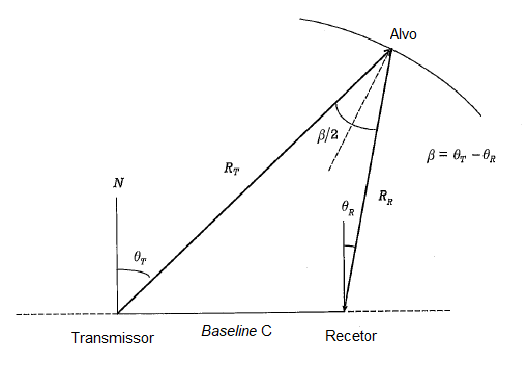
\includegraphics[scale=0.9]{chapters/ch2/assets/geom}
\caption[Parâmetros na geometria bistática]{Parâmetros na geometria bistática (Adaptada de \cite{GRIFFITHS2014813})}
\label{fig:geom}
\end{figure}

O termo alcance bistático, ou \textit{bistatic range}, é definido em \ref{2.1} \parencite{Griffiths2017}. Com este valor é possível criar elipses bistáticas (para duas dimensões) ou elipsoides bistáticos (para três dimensões) com o transmissor e o recetor como dois focos das mesmas. \par

\begin{equation} \label{2.1} 
R_{T}+R_{R}-C 
\end{equation}

Contudo, se a \textit{baseline} $C$ for um valor conhecido, pode-se extrair o termo \textit{range sum} $R_{T}+R_{R}$. \par
Através do conhecimento do valor de $\theta_{R}$, que é mensurável se a antena de \textit{surveillance} for direcional, a distância do alvo ao recetor é dada pela expressão \ref{2.2}.

\begin{equation} \label{2.2}
R_{R}=\dfrac{\left(  R_{T}+R_{R}\right)^{2}-C^{2}}{2\left(  R_{T}+R_{R}+C sin\theta_{R}\right)}
\end{equation}


Um dos parâmetros importantes quando no alcance bistático é a \textit{range resolution}, ou seja, a resolução em alcance. Este parâmetro é definido pela capacidade de distinguir os alvos que estão muito próximos. Um exemplo de um sistema radar que necessite de boa \textit{range resolution} é um sistema de direção de tiro. \par 

Num radar convencional monostático, a resolução em alcance é dada por $\delta_{R}=c/2B$, onde c é a velocidade de propagação e B a largura de banda do sinal transmitido. No entanto, num radar passivo, a geometria é bistática, o que leva a existirem diferentes elipses bistáticas concêntricas, isto é, com centro no mesmo ponto, o que tem de ser tomado em conta na expressão que representa a \textit{range resolution}:

\begin{equation} \label{2.3}
\delta_{r}=\dfrac{c}{2B\left( cos\dfrac{\beta}{2}\right)}
\end{equation}

No entanto, este caso é específico para quando os dois alvos estão alinhados relativamente à bissetriz do ângulo $\beta$, como é possivel observar na figura \ref{fig:geom_varios_alvos} o exemplo dos alvos 1 e 2. Para um caso generalizado, como por exemplo o alvo 1 e o alvo 3, a expressão da \textit{bistatic range resolution} (Expressão \ref{2.4}) depende de mais um valor $\varphi$ representado na figura \ref{fig:geom_varios_alvos} como o ângulo entre o seguimento da bissetriz do ângulo $\beta$ e o segmento de reta que une o alvo 1 e o alvo 3 com centro no alvo 1. 

\begin{figure}[h]
\centering
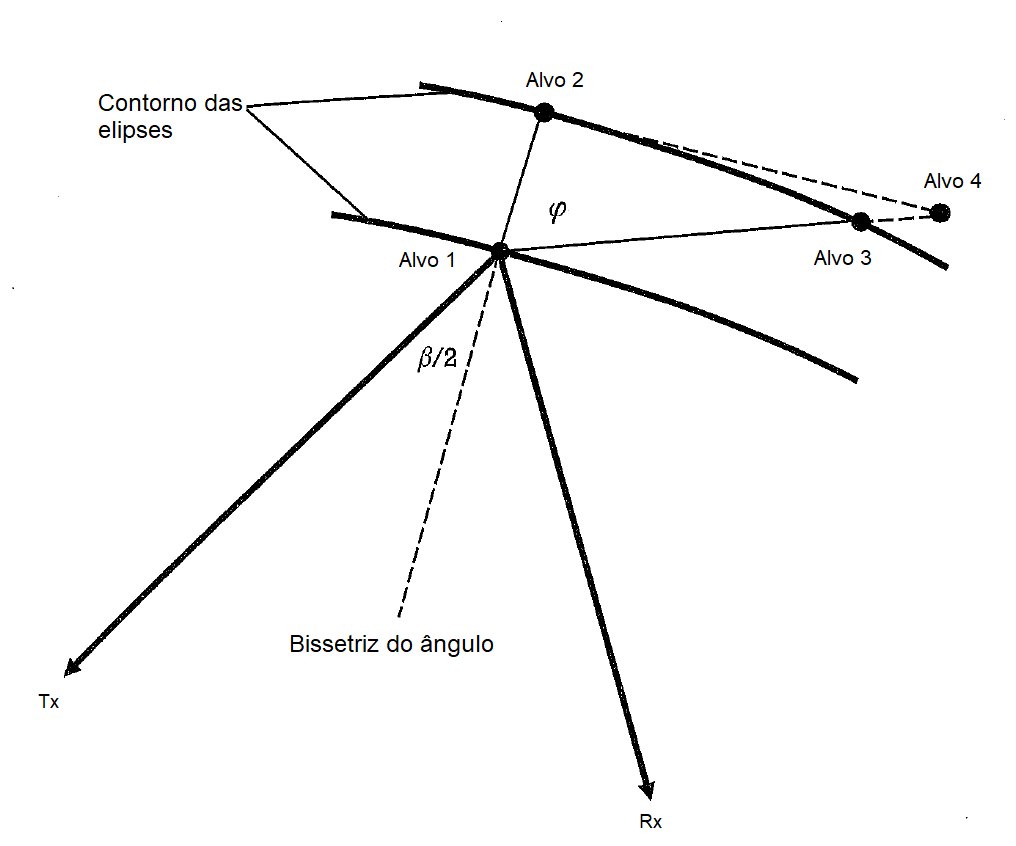
\includegraphics[scale=0.5]{chapters/ch2/assets/geom_varios_alvos}
\caption[Geometria bistática para vários alvos]{Geometria bistática para vários alvos (Adaptada da figura 2.4 \cite{Griffiths2017})}
\label{fig:geom_varios_alvos}
\end{figure}


\begin{equation} \label{2.4}
\delta_{r}=\dfrac{c}{\left[ 2B\left( cos\dfrac{\beta}{2}\right)\right] cos\varphi}
\end{equation}


A expressão do \textit{bistatic range resolution} permite interpretar a geometria bistática quanto à distância entre o transmissor e recetor. Da expressão \ref{2.4} conclui-se que quanto mais o ângulo $\beta$ se aproxima de um ângulo reto, o denominador tende para um valor próximo de 0, ou seja, a resolução em alcance torna-se fraca. Contudo, nesta situação estamos perante uma geometria \textit{forward scatter}, discutido no inicio deste capítulo, o que pode ser contornando usando vários recetores em locais diferentes.\par 
Para radares passivos, continuando a interpretação da expressão \ref{2.4}, os iluminadores de oportunidade mais utilizados têm pouca largura de banda $B$, o que se reflete na diminuição da resolução em alcance. No entanto, os sinais de \gls{DVB-T}, discutidos no Capítulo \ref{chap:Chapter1}, têm uma largura de banda na ordem dos $8 MHz$, o que permite uma resolução em alcance na ordem dos $40m$.

\subsubsection*{\textit{Doppler}} 
Ignorando efeitos relativisticos, o desvio de \textit{Doppler} bistático ocorre quando pelo menos um dos elementos transmissor, alvo, recetor se encontra em movimento. É definido como a taxa de variação temporal do comprimento total do caminho percorrido pelo sinal refletido, normalizado pelo comprimento de onda $\lambda$ \parencite{Willis2005}.  No caso mais comum, em que apenas o alvo se encontra em movimento, o desvio de \textit{Doppler} é dado por \parencite{Willis2005},

\begin{equation} \label{2.5}
f_{D}=\dfrac{2v}{\lambda}cos\delta cos\left( \dfrac{\beta}{2}\right) 
\end{equation}

onde $\delta$ é o ângulo formado pelo sentido do vetor velocidade $v$ e a bissetriz do ângulo $\beta$ com centro no alvo. \par

Na equação \ref{2.5}, quando $\beta =180^{\circ}$, estamos perante uma geometria \textit{forward scatter} e temos um valor de desvio de \textit{Doppler} $f_{D}=0$ para todos os ângulos de $\delta$. Quando $\beta =0^{\circ}$, fica-se reduzido a uma geometria monostática. 


A resolução de \textit{Doppler} no radar bistático é semelhante à resolução de \textit{Doppler} no radar monostático, isto porque depende do tempo de integração $T$ que é um parâmetro escolhido e indiferente à geometria do radar. Quanto maior for o tempo de integração, melhor é a resolução de \textit{Doppler}. A expressão \ref{2.6} define o requisito mínimo entre a separação dos alvos.

\begin{equation} \label{2.6}
\vert f_{a1}-f_{a2}\vert = \dfrac{1}{T}
\end{equation}

sendo que $f_{a1}$ e $f_{a2}$ são os desvios de \textit{Doppler} para cada alvo, definidos em \ref{2.5}. Substituindo as equações dos alvos em \ref{2.5} na equação \ref{2.6}, e resolvendo em ordem a $\Delta v$, ou seja, a diferença entre os dois vetores velocidade projetados na bissetriz do ângulo $\beta$ ($\Delta v=\left( v_{1}cos\delta_{1}-v_{2}cos\delta_{2}\right) $), vem,

\begin{equation} \label{2.7}
\Delta v = \dfrac{\lambda}{2T\cdot cos\left( \beta /2\right) }
\end{equation}

Com esta expressão, assumimos que os alvos partilham a mesma bissetriz, o que na realidade é pouco provável. No entanto, esta restrição pode ser ignorada, se,
\begin{enumerate}
	\item A separação entre os alvos não for suficiente para permitir resolução em \textit{range};
	\item O ângulo entre as bissetrizes dos dois alvos é pequeno.
\end{enumerate}



\subsection{Previsão de Desempenho}
Para qualquer sistema radar é importante conseguir prever com precisão os vários aspetos do desempenho do sistema. O ponto de início de uma análise de desempenho do radar passivo é a equação de radar bistática, referida brevemente no capítulo \ref{chap:Chapter3} e rescrita  de uma forma que reflete as caraterísticas do radar \gls{PCL} para o caso da geometria bistática vem \parencite{Griffiths2005},

\begin{equation} \label{2.8}
\dfrac{P_{r}}{P_{n}}= \dfrac{P_{t}G_{t}}{4\pi r^{2}_{1}}\cdot\sigma_{b}\cdot\dfrac{1}{4\pi r^{2}_{2}}\cdot\dfrac{G_{r}\lambda^{2}}{4\pi}\cdot\dfrac{1}{kT_{0}BF}\cdot L 
\end{equation}

onde,\par
$P_{r}$: "potência do sinal recebido"\par
$P_{n}$: "potência do ruído do recetor"\par
$P_{t}$: "potência do sinal transmitido"\par
$G_{t}$: "ganho da antena de transmissão"\par
$G_{r}$: "ganho da antena de receção"\par
$r_{1}$: "alcance do transmissor ao alvo"\par
$r_{2}$: "alcance do recetor ao alvo"\par
$\sigma_{b}$: "\gls{RCS} bistática do alvo"\par
$\lambda$: "comprimento de onda do sinal"\par
$k$: "constante de \textit{Boltzmann}$ =1,380649x10^{-23} J\cdot K^{-1}$"\par
$T_{0}$: "temperatura de ruído de referência, $290K$"\par
$B$: "largura de banda efetiva do recetor"\par
$F$: "\textit{noise figure}\footnote{\textit{noise figure} ou figura de ruído representa a diferença em $dB$ entre o ruído de entrada do recetor e a ruído de saída do mesmo} efetiva do recetor"\par
$L(\leq 1)$: "perdas do sistema"\par
 
É de notar que para esta equação, usada para a previsão de \textit{peformance}, é importante conhecer o valor de cada parâmetro a ser usado, o que leva a ter uma ideia bem definida da função do sistema radar e o que se pretende com o mesmo. Também é necessário o conhecimento dos vários iluminadores de oportunidade e as suas caraterísticas, referido no subcapítulo \ref{IOS}.\par 


\subsubsection*{Potência transmitida}
A potência transmitida $P_{t}$ é substancial para muitas das fontes de sinal para o radar passivo devido aos recetores de sinais de \textit{broadcast} e comunicações apresentarem, normalmente, antenas ineficientes e com \textit{noise figures} baixas. Isto é, as antenas de receção dos sinais mais comuns no espetro, são antenas que têm de ser relativamente baratas, por exemplo uma antena de receção de \gls{DVB-T} ou de receção de radiodifusão sonora em \gls{VHF}, de forma a o utilizador comum poder ter acesso a qualquer uma destas, logo este tipo de antenas são mais ineficientes e isso é colmatado por uma maior potência de transmissão por parte da estação de difusão.\par 
Seja qual for o iluminador de oportunidade utilizado, a potência do transmissor interfere com a densidade de potência $\Phi =(P_{t}G_{t})/4\pi r^{2}_{1}$, que é uma caraterística importante na escolha da fonte de sinal a ser utilizada. 

\subsubsection*{\gls{RCS} bistática do alvo}
Na deteção de alvos usando radares \gls{PCL}, a \gls{RCS} bistática do alvo é uma caraterística importante na previsão de desempenho. As caraterísticas do alvo definem este parâmetro e também a sua localização em relação ao transmissor - recetor, formando o ângulo bistático $\beta$, referido no ínicio deste capítulo. É dificil ter uma previsão deste parâmetro, mas há um caso especial a ser considerado, que é para uma geometria \textit{forward scatter}. \par 
Quando o ângulo bistático, representado na figura \ref{fig:geom} por $\beta$, toma valores próximos de $180^{\circ}$, entra-se na região de \textit{forward scatter} e nesta zona, o valor da \gls{RCS} do alvo é melhorado devido ao principio de \textit{Babinet}. Este principio aplicado a este caso, diz que para um alvo que é um absorvedor perfeito, na região de \textit{forward scatter}, a dispersão de energia que é transmitida para o recetor é igual à dispersão que era transmitida se no lugar deste alvo estivesse presente uma abertura com a mesma forma \parencite{Griffiths2005}. Assim sendo, para um alvo com uma área transversal $A$, a \gls{RCS} é representada na equação \ref{2.9} e a largura de feixe do sinal refletido na equação \ref{2.10}.

\begin{equation} \label{2.9}
\sigma_{b}=\dfrac{4\pi A^{2}}{\lambda^{2}}
\end{equation}

\begin{equation} \label{2.10}
\theta_{b}=\dfrac{\lambda}{d}
\end{equation}

Onde $d$ é a dimensão linear no plano apropriado.
Ao analisar as duas funções fazendo variar a frequência (a partir da figura \ref{fig:rcs_ang}) é de notar que com menor frequência consegue-se menor largura de feixe e maior \gls{RCS} bistática do alvo. Isto fundamenta o uso de radares com frequência baixa para a deteção na zona de \textit{forward scatter}.

\begin{figure}[h]
\centering
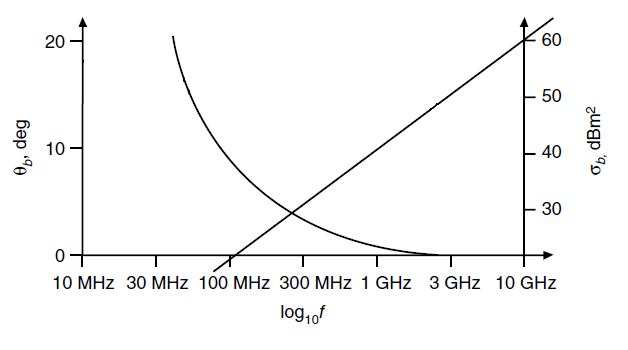
\includegraphics[scale=0.7]{chapters/ch2/assets/rcs_ang}
\caption[Variação da \gls{RCS} e largura de feixe consoante a frequência]{Variação da \gls{RCS} e largura de feixe consoante a frequência, para um alvo de $10m^{2}$ de área e dimensão linear $20m$ (figura 1 \cite{Griffiths2005})}
\label{fig:rcs_ang}
\end{figure}

\subsubsection*{\textit{Noise figure} do recetor}
A \textit{noise figure} , de uma forma simples, é definida pela relação entre a \gls{SNR} à entrada do recetor e a \gls{SNR} à saída do mesmo, ou seja, é um valor que representa o desempenho do recetor, sendo que quanto menor for, mais perto se encontram os dois valores de \gls{SNR} e consequentemente melhor desempenho.\par
Não é só a \textit{noise figure} que contribui para os níveis de ruído presentes no sinal. Por forma a compreender melhor os fatores que contribuem para os níveis de ruído, pode ser criada uma função $P_{i}(\theta ,f)$ dependente da direção e frequência que engloba todos estes fatores, sendo estes:
\begin{enumerate}
\item \textit{Noise figure} do recetor;
\item Sinal direto do transmissor, que é a componente mais forte desta função;
\item Componente de \textit{multipath}, ou seja, todas as réplicas do sinal direto atrasadas no tempo devido a reflexões em obstáculos;
\item Sinal direto e \textit{multipath} de outros sinais que possam estar a transmitir no mesmo canal;
\item Outros sinais devido a fontes diversas, como por exemplo radiação de dispositivos eletrónicos.
\end{enumerate}
Devido a todas estas componentes é necessário haver um cancelamento das mesmas de forma a ser percetível o sinal refletido no alvo e aumentar a sensibilidade e alcance do sistema. No capítulo \ref{chap:Chapter4} é abordado este assunto com mais pormenor.\par 

A \textit{noise figure} do recetor, pode ser representada pela seguinte equação,

\begin{equation} \label{2.11}
NF=10log_{10}\left( \dfrac{SNR_{i}}{SNR_{o}}\right)=SNR_{i,dB}-SNR_{o,dB}
\end{equation}

\subsubsection*{Ganho de integração}
A largura de banda efetiva do recetor $B$, que é normalmente a largura de banda do sinal transmitido, é adaptada ao sinal direto e, quando combinada com um tempo de integração $T$, resulta um ganho de integração como representado na equação \ref{2.12}. Este tempo de integração é referido no capítulo \ref{chap:Chapter4} como o tempo em que é integrada a relação cruzada.

\begin{equation} \label{2.12}
G_{i}=BT
\end{equation}

Para o caso da \gls{DVB-T}, que a largura de banda é aproximadamente $8 MHz$, com um tempo de integração de 1 segundo dá um ganho de processamento $G_{i}$ de $69dB$, o que se torna muito melhor que o ganho de integração de por exemplo uma transmissão rádio \gls{FM} com uma largura de banda de $50 kHz$, que para 1 segundo de tempo de integração vem um ganho de $47dB$.\par 
Tendo como referência a equação \ref{2.12}, podemos ter a perceção de que para obter maior ganho de integração num determinado sinal, basta aumentar o tempo de integração da correlação para valores maiores, o que é verdade, mas ao fazer isto, existem vários efeitos limitativos que vão ocorrer. Um dos principais efeitos mais limitativo é conhecido como \textit{target flutuations}, ou seja, alterações repentinas da força do sinal, que é resultante de maioritariamente dois fatores: a mudança de ângulo de observação e o efeito de \textit{multipath}. Com isto, a função do ganho de integração já não vai ser linear e aumentar sempre com o aumento do tempo de integração, pelo oposto, dependendo de vários fatores vai ter um pico para um determinado tempo de integração.\par 
Este tema tem sido estudado e foram tiradas várias conclusões com resultados de alvos reais \parencite{Malanowski2008}. Uma das conclusões que foi verificada, foi que o tempo de integração da correlação é importante para ecos fracos, que são originados por reflexões em alvos distantes e que para alvos mais próximos, normalmente existe boa \gls{SNR} e não é necessário maior tempo de integração. Também são abordadas e testadas soluções para este problema usando diferentes versões da função de correlação.

\subsubsection*{Previsão de \textit{performance} na deteção}
Como conclusão deste subcapítulo e depois da abordagem em alguns tópicos considerados mais importantes na previsão de \textit{performance} de um radar passivo são apresentados exemplos práticos \parencite{Griffiths2005} de uma previsão de alcance para dois transmissores de rádio \gls{FM} localizados em Wrotham e Crystal Palace, com o recetor localizado no edifício \textit{Engineering Sciences Faculty} da \gls{UCL}.

\begin{figure}[h]
\centering
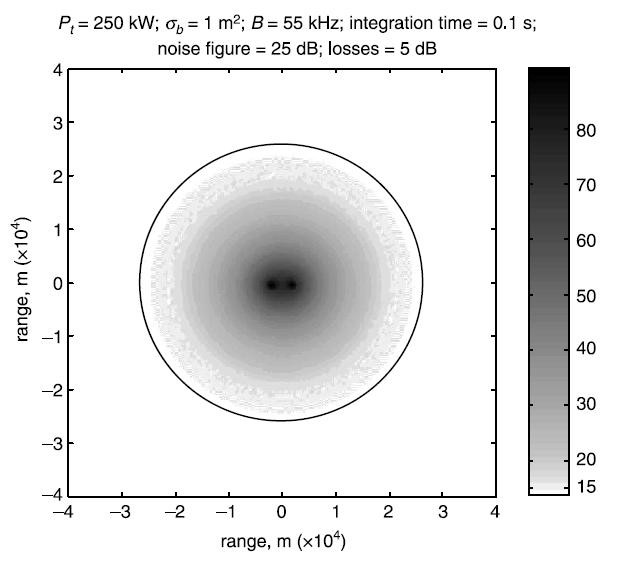
\includegraphics[scale=0.6]{chapters/ch2/assets/wrotham}
\caption[Alcance de deteção para um transmissor em Wrotham e recetor na \gls{UCL}]{Alcance de deteção para um transmissor em Wrotham e recetor na \gls{UCL} (figura 3 \cite{Griffiths2005})}
\label{fig:wrotham}
\end{figure}

\begin{figure}[h]
\centering
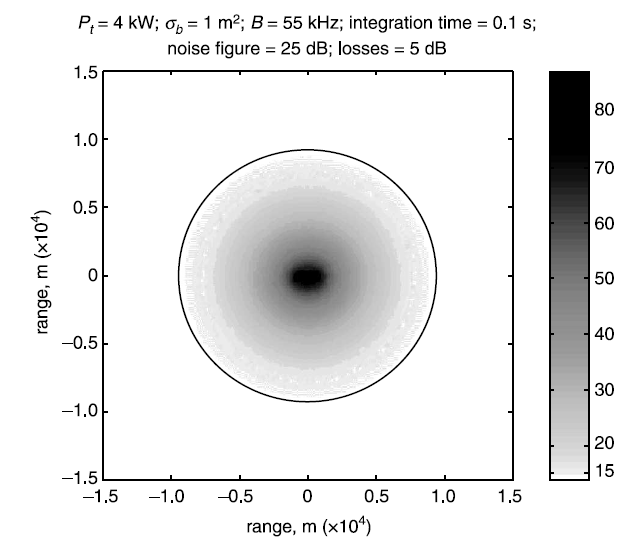
\includegraphics[scale=0.6]{chapters/ch2/assets/cp}
\caption[Alcance de deteção para um transmissor em Crystal Palace e recetor na \gls{UCL}]{Alcance de deteção para um transmissor em Crystal Palace e recetor na \gls{UCL} (figura 4 \cite{Griffiths2005})}
\label{fig:cp}
\end{figure}

Várias observações podem ser feitas com estas duas figuras, mas a primeira que se sobressai é o alcance de deteção para um transmissor, sendo que a linha preta que contorna os dois transmissores é uma referência para os $15dB$, que ronda pouco mais de $10km$ para o transmissor em Crystal Palace, e para o transmissor em Wrotham o já está na ordem dos $30km$. Isto deve-se à potência de transmissão, que no caso de Crystal Palace é de $4kW$ e em Wrotham, $250kW$, o que leva de novo a um dilema que tem sido debatido ao longo desta dissertação, que é a escolha do iluminador de oportunidade e a variedade de fatores que afetam esta escolha nunca conseguindo ter uma fonte de sinal ideal, mas sim uma mais adaptada à função do radar passivo.


\subsection{Formação de Imagem}
O radar \gls{PCL}, ou radar passivo, não oferece apenas a capacidade de explorar os iluminadores de oportunidade para o fim de deteção e localização, mas também para a formação de imagens. Tem muitas vantagens na utilização deste tipo de radares para este fim, sendo um bom exemplo o mapeamento de uma zona com qualquer condição meteorológica e sem transmitir nenhum sinal.\par 
O objetivo deste subcapítulo é dar um conhecimento superficial sobre uma das capacidades dos radares passivos e dar a conhecer alguns conceitos fundamentais e um algoritmo \gls{PB-ISAR} na formação de imagens.\par 

\subsubsection*{\gls{ISAR}}
O conceito do \gls{ISAR} é utilizar uma configuração de um radar de abertura sintética, mas em que o radar esteja estático e o alvo em movimento em relação ao mesmo (Inverso do \gls{SAR}). Ao utilizar esta abordagem é necessário criar uma abertura sintética por forma a ter boa resolução \textit{cross-range}, que é conseguida, no caso do \gls{SAR}, por um elemento que se move ao longo de uma trajetória conseguindo assim meios para formar uma matriz virtual para o intervalo de tempo em que esteve a observar. O único caso em que esta matriz virtual criada pela abertura sintética é diferente de uma imagem obtida por uma matriz real é quando o espaço a ser iluminado está estático em relação ao radar durante a formação da mesma.\par 
Os elementos chave para a construção de uma imagem usando \gls{ISAR} são \parencite{Martorella2019}:

\begin{enumerate}
\item Utilizar um sinal com grande largura de banda por forma a ter uma boa resolução em \textit{range} $\delta_{R}$ falado no subcapítulo \ref{subchapter:alcance_bistatico} para o caso monostático e bistático.

\item Processar os ecos recebidos durante o tempo de observação em diferentes ângulos de incidência no alvo a iluminar. A resolução \textit{cross-range} é definida na equação \ref{2.13}, que é inversamente proporcional à variação de ângulo de incidência $\Delta$.
\begin{equation} \label{2.13}
\delta_{cr}=\dfrac{c}{2f_{0}\Delta}
\end{equation}
\end{enumerate}

Por forma a compreender o processo de formação de imagem de uma forma simples, segue-se o diagrama de blocos da figura \ref{fig:img}. Este diagrama não compreende todos os processos englobados na formação de imagem através de \gls{ISAR}, mas apenas os fundamentais para uma breve explicação que é o objetivo deste subcapítulo.

\begin{figure}[h]
\centering
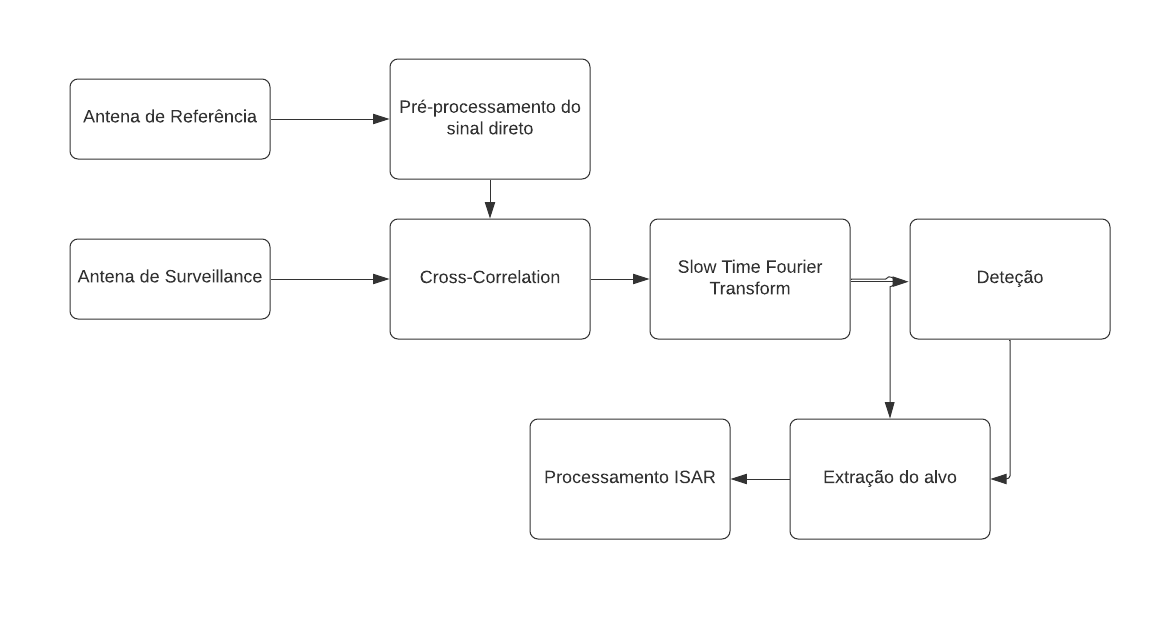
\includegraphics[scale=0.8]{chapters/ch2/assets/img}
\caption[Diagrama de blocos ISAR]{Diagrama de blocos ISAR}
\label{fig:img}
\end{figure}

Depois de recebido o sinal da antena de referência e \textit{surveillance} o sinal direto é submetido a um pré processamento explicado no capítulo \ref{chap:Chapter4} que para o caso de \gls{DVB-T} visto que é um dos iluminadores de oportunidade com maior largura de banda o que permite maior resolução em \textit{range}, reconstrução e equalização do sinal. Esse sinal direto passa por um equivalente a um filtro adaptado, ou seja, a \textit{cross-correlation} do sinal direto com o sinal refletido no alvo.\par 

O \textit{input} do algoritmo \gls{PB-ISAR} é um mapa \textit{range-Doppler} que contém o eco do alvo mais \textit{clutter} e ruído. No entanto, os radares do tipo \gls{ISAR} são desenvolvidos para trabalhar no domínio frequência/\textit{slow-time} ou \textit{range}/\textit{slow-time} e para isso ser possível é necessário transformar os dados recebidos do mapa \textit{range-Doppler} num destes domínios. Uma das formas para o fazer, no caso de transformar no domínio frequência/\textit{slow-time} é aplicar uma transformada de \textit{Fourier} inversa à imagem em \textit{range-Doppler} do alvo.\par 

Após este processamento, que no caso do filtro adaptado é explicado sucintamente no capítulo \ref{chap:Chapter4}, o sinal passa por um bloco de extração do alvo que consiste em quatro passos:
\begin{enumerate}
\item processo de \textit{clustering} dos alvos detetados no mapa \textit{range-Doppler} com um exemplo representado na imagem \ref{fig:cluster};

\begin{figure}[h]
\centering
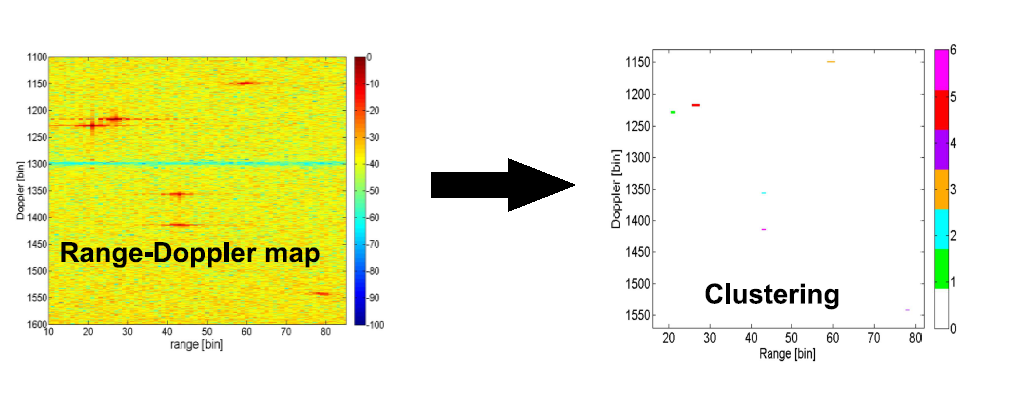
\includegraphics[scale=0.6]{chapters/ch2/assets/cluster}
\caption[Processo de \textit{clustering}]{Processo de \textit{clustering} (adaptado da figura do slide 36 da apresentação do artigo \cite{Martorella2019})}
\label{fig:cluster}
\end{figure}

\item criação de uma caixa em redor do alvo;
\item através das caixas formadas em redor dos alvos, resolver possíveis problemas de \textit{overlapping} e desviar erros de deteção de vários alvos próximos quando na realidade apenas se encontra um;
\item extração dos alvos detetados.
\end{enumerate}

De seguida a imagem passa por um pré-processamento do \gls{ISAR} por forma a definir perfis de \textit{range} em cada alvo extraído que, por fim, é submetida ao processamento do \gls{ISAR} onde é feito uma estimativa a partir do pré-processamento da posição dos alvos em relação ao recetor e, posteriormente uma compensação do movimento do alvo seguida de uma \gls{DFT} para obter a imagem \gls{ISAR} do alvo. Para um entendimento mais profundo dos cálculos e processamento, tanto como resultados obtidos com este métodos há vários trabalhos que se podem consultar como \cite{Martorella2019}.